\section{Byte Latent Transformer (BLT)}
\begin{frame}{}
    \LARGE \textbf{Byte Latent Transformer (BLT)}
\end{frame}

\begin{frame}[allowframebreaks]{Byte Latent Transformer (BLT)}
    \begin{figure}
        \centering
        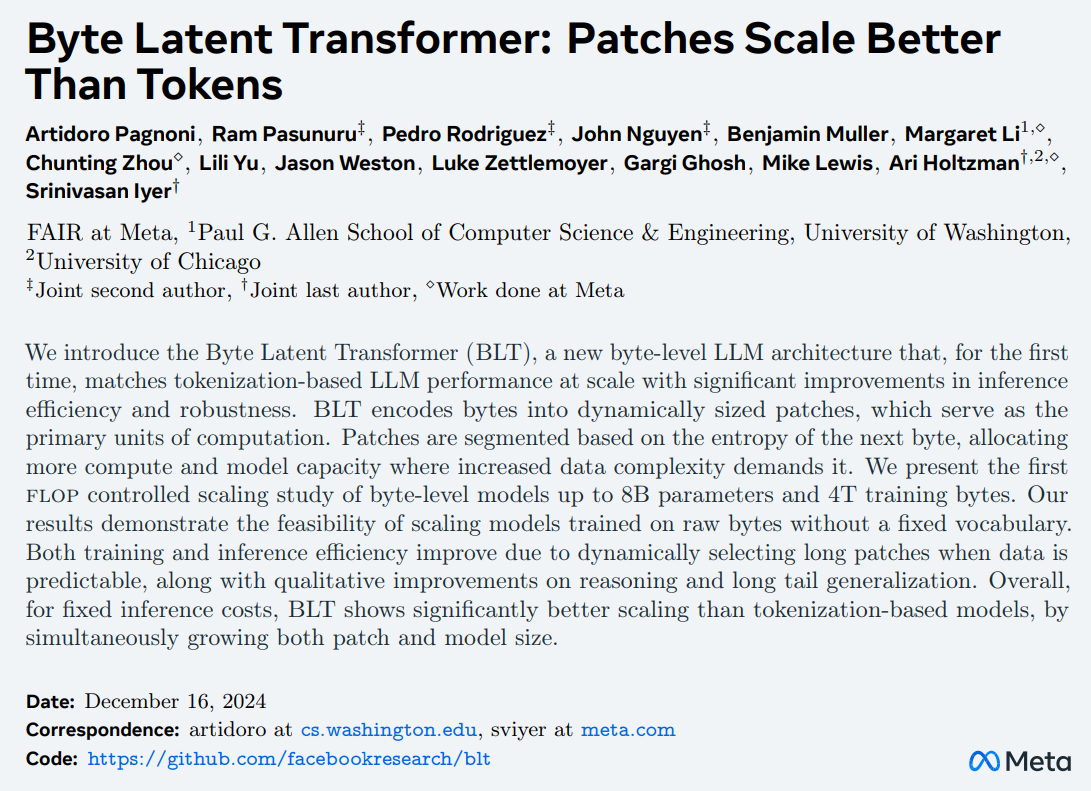
\includegraphics[height=0.9\textheight,width=1.05\textwidth,keepaspectratio]{images/recent-advance/blt-paper.png}
    \end{figure}

\framebreak
    \textbf{BLT} is a compression-based approach for efficient LLMs:
    \begin{itemize}
        \item Compress input text into a smaller latent space
        \item Run transformer on latent tokens
        \item Decode with a decoder-only model
    \end{itemize}
    \vspace{1em}
    \begin{itemize}
        \item[\checkmark] Reduces memory \& compute
        \item[\checkmark] Maintains quality (BLEU, perplexity)
        \item[\checkmark] Works well with long context (128k+)
    \end{itemize}
    \vspace{1em}
    \textbf{Related:} VQ-VAE, tokenizer-free models, compression transformers
    \vspace{1em}
    \footnotesize{\textbf{Meta AI (2024)} \url{https://ai.meta.com/research/publications/byte-latent-transformers-compression-based-efficiency-for-byte-level-llms/}}
\framebreak
    \begin{figure}
        \centering
        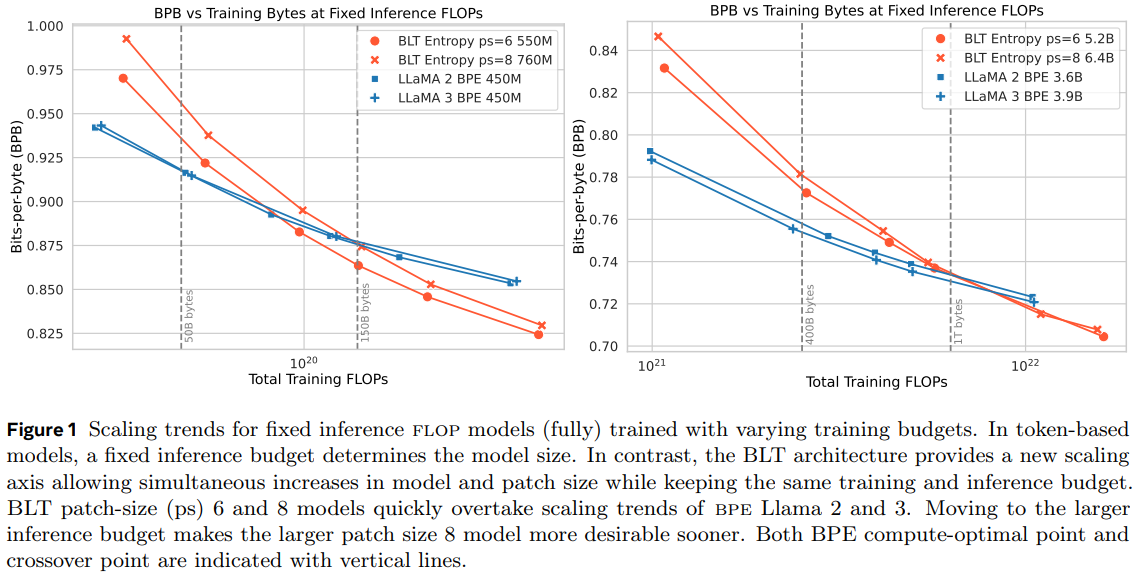
\includegraphics[height=0.9\textheight,width=1.05\textwidth,keepaspectratio]{images/recent-advance/blt-flops.png}
    \end{figure}
\framebreak
    \begin{figure}
        \centering
        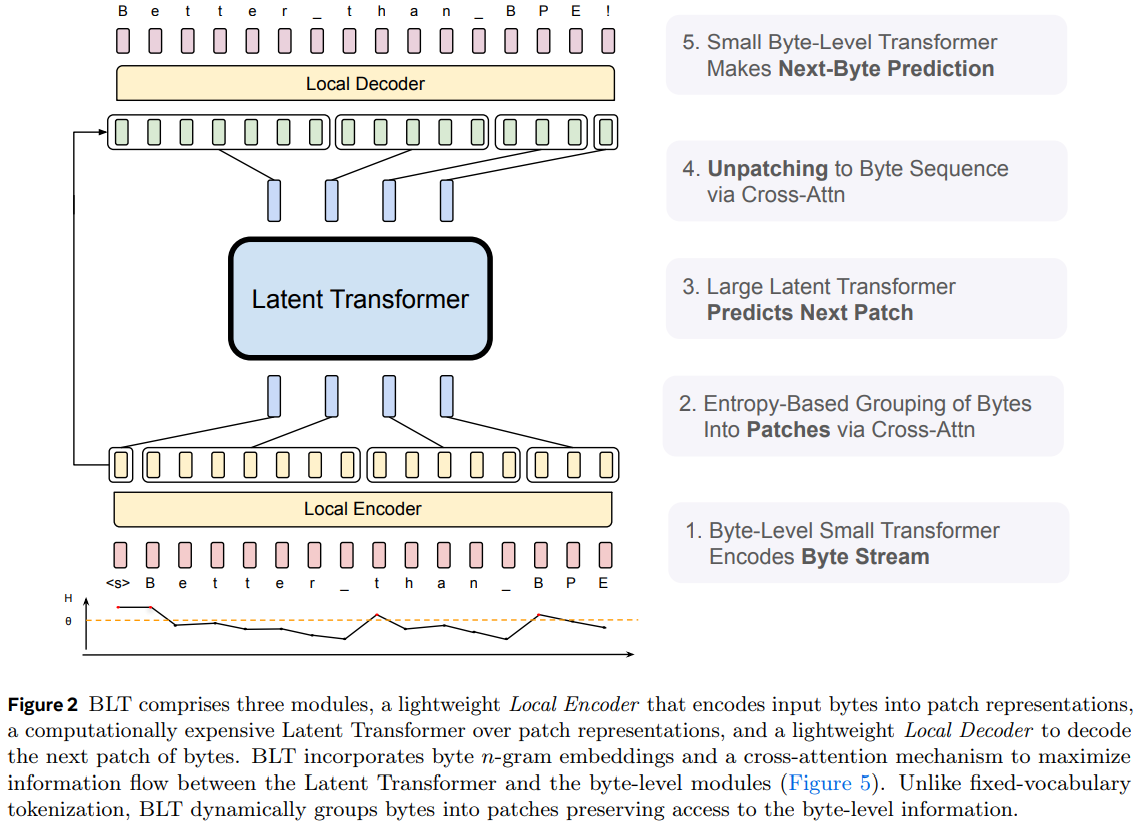
\includegraphics[height=0.9\textheight,width=1.05\textwidth,keepaspectratio]{images/recent-advance/blt-modules.png}
    \end{figure}
\framebreak
    \begin{figure}
        \centering
        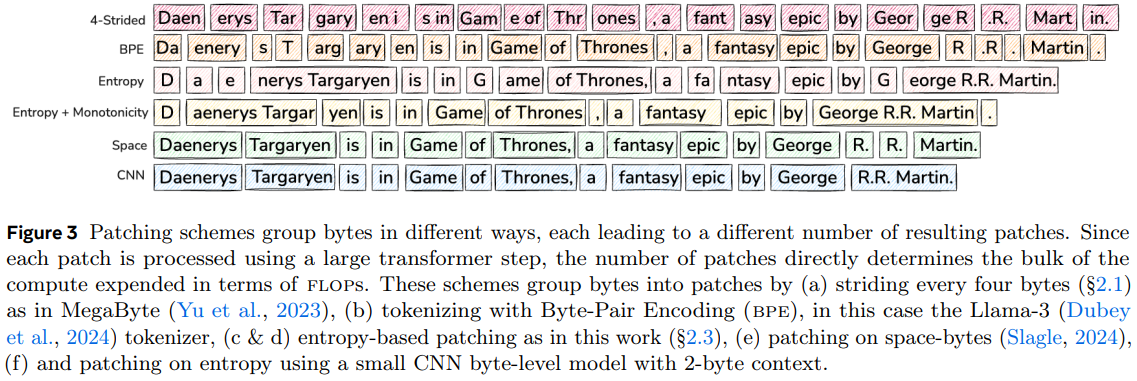
\includegraphics[height=0.9\textheight,width=1.05\textwidth,keepaspectratio]{images/recent-advance/blt-patch-scheme.png}
    \end{figure}
\framebreak
    \begin{figure}
        \centering
        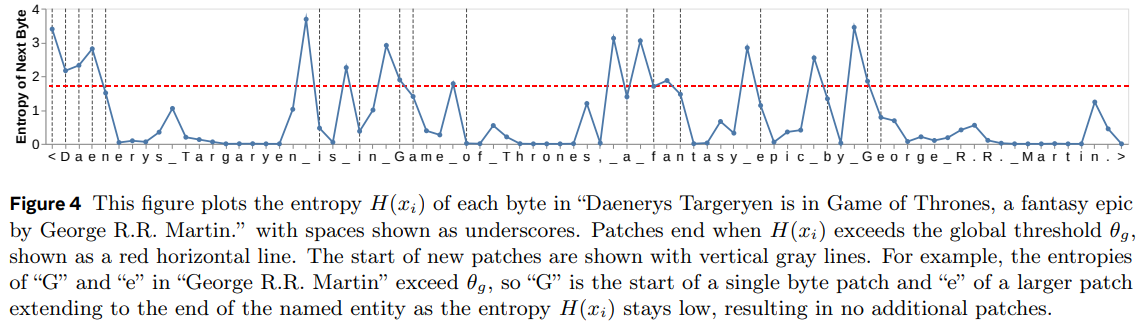
\includegraphics[height=0.9\textheight,width=1.05\textwidth,keepaspectratio]{images/recent-advance/blt-entropy.png}
    \end{figure}
\end{frame}

\begin{frame}[allowframebreaks]{Space Patching}
    \textbf{Space Patching} (Slagle, 2024) improves over strided patching by creating new patches after any space-like byte, which often aligns with word boundaries in many languages.
    \begin{itemize}
        \item Allocates a latent transformer step for every word.
        \item Ensures consistent patching of words across sequences.
        \item Focuses compute (flops) on hard predictions, typically following spaces.
    \end{itemize}
    \vspace{1em}
    \textbf{Example:} Predicting the first byte of the answer to “Who composed the Magic Flute?” is harder than predicting subsequent bytes in “Mozart”.
    \begin{itemize}
        \item The first character narrows down possible completions, making the rest easier to predict.
    \end{itemize}
\framebreak
    \textbf{Limitations:}
    \begin{itemize}
        \item Not suitable for all languages or domains.
        \item Cannot vary patch size.
    \end{itemize}
    \vspace{1em}
    \textbf{Next:} A new patching method that leverages the difficulty of predicting initial bytes in words and enables control over patch size.
\end{frame}

\begin{frame}[allowframebreaks]{Entropy Patching}
    \textbf{Entropy Patching: Using Next-Byte Entropies from a Small Byte LM}
    \begin{itemize}
        \item Instead of rule-based heuristics (e.g., whitespace), entropy patching uses a data-driven approach to identify high-uncertainty next-byte predictions.
        \item Train a small byte-level auto-regressive LM on BLT training data.
        \item Compute next-byte entropies $H(x_i)$ under the LM distribution $p_e$ over the byte vocabulary $V$:
    \end{itemize}
    \begin{equation}
        H(x_i) = -\sum_{v \in V} p_e(x_i = v \mid x_{<i}) \log p_e(x_i = v \mid x_{<i})
    \end{equation}
\framebreak
    \begin{itemize}
        \item Two methods for identifying patch boundaries:
        \begin{enumerate}
            \item \textbf{Global Constraint:} $H(x_t) > \theta_g$ (entropy above a global threshold)
            \item \textbf{Approx. Monotonic Constraint:} $H(x_t) - H(x_{t-1}) > \theta_r$ (entropy rises relative to previous byte)
        \end{enumerate}
        \item The second method finds points that break approximate monotonically decreasing entropy within a patch.
        \item Patch boundaries are identified during lightweight preprocessing at dataloading.
        \item Differs from Nawrot et al. (2023), which trains a classifier to predict entropy-based patch boundaries.
    \end{itemize}
    \vspace{1em}
    \textbf{In experiments:} Both methods are compared for distinguishing between low and high entropy bytes.
\end{frame}

\begin{frame}[allowframebreaks]{Encoder Multi-Headed Cross-Attention}
    \textbf{Encoder Multi-Headed Cross-Attention:}
    \begin{itemize}
        \item Follows Perceiver input cross-attention (Jaegle et al., 2021), but latent representations correspond to variable patch representations (not fixed set).
        \item Each patch $p_j$ attends only to its own bytes.
        \item Query vector for each patch is initialized by pooling byte representations for $p_j$, then projecting via $EC \in \mathbb{R}^{h_E \times (h_E \times U_E)}$, where $U_E$ is the number of encoder cross-attention heads.
    \end{itemize}
    \vspace{1em}
    \textbf{Formulation:}
    \begin{align}
        P_{0,j} &= EC(f_{\text{bytes}}(p_j)) \quad \text{(Pooling function $f$ over bytes in patch $p_j$)} \\
        P_l &= P_{l-1} + W_o \left[ \mathrm{softmax} \left( \frac{Q K^T}{\sqrt{d_k}} \right) V \right] \\
        Q_j &= W_q(P_{l-1,j}) \\
        K_i &= W_k(h_{l-1,i}) \\
        V_i &= W_v(h_{l-1,i}) \\
        h_l &= \text{Encoder-Transformer-Layer}_l(h_{l-1})
    \end{align}
    \vspace{1em}
    \begin{itemize}
        \item $P \in \mathbb{R}^{n_p \times h_G}$: $n_p$ patch representations for the global model.
        \item $W_q$, $W_k$, $W_v$, $W_o$: learned projection matrices.
        \item Patch representations are initialized by pooling byte embeddings $e_i$ for each patch $p_j$.
    \end{itemize}
    \vspace{1em}
    \textbf{Key Difference:} Latent representations are variable and correspond to patch boundaries, not a fixed latent set.
\framebreak
    \begin{figure}
        \centering
        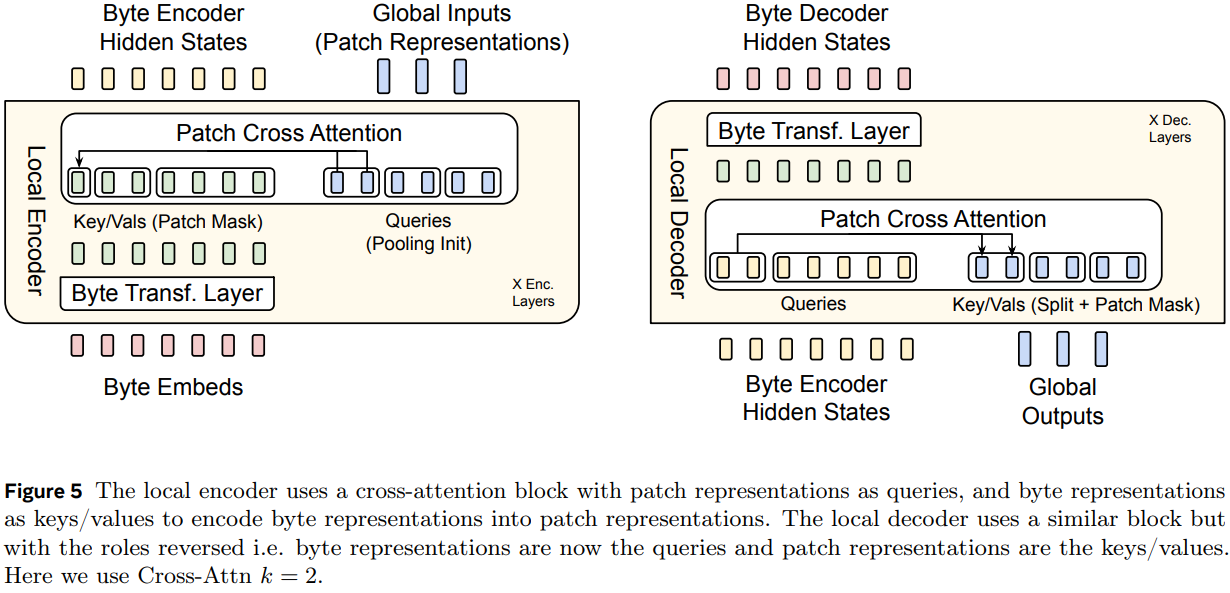
\includegraphics[height=0.9\textheight,width=1.05\textwidth,keepaspectratio]{images/recent-advance/blt-cross-attention.png}
    \end{figure}
\end{frame}

\begin{frame}[allowframebreaks]{Decoder Multi-Headed Cross-Attention}
    \textbf{Decoder Multi-Headed Cross-Attention:}
    \begin{itemize}
        \item In the decoder, the roles of queries and key/values are swapped compared to the encoder cross-attention.
        \item Byte representations act as queries, while patch representations serve as keys and values.
        \item Initial byte representations for cross-attention are set as the byte embeddings from the last encoder layer, $h^E$.
    \end{itemize}
    \vspace{1em}
    \textbf{Formulation:}
    \begin{align}
        D_0 &= h^E \\
        B_l &= D_{l-1} + W_o \left[ \mathrm{softmax} \left( \frac{Q K^T}{\sqrt{d_k}} \right) V \right] \\
        Q_i &= W_q(d_{l-1,i}) \\
        K_j &= W_k(DC(o_j)) \\
        V_j &= W_v(DC(o_j)) \\
        D_l &= \text{Decoder-Transformer-Layer}_l(B_l)
    \end{align}
    \begin{itemize}
        \item $DC$ is a linear transformation and split operation applied to the final patch representations $o_j$ from the global model.
        \item $W_q$, $W_k$, $W_v$, $W_o$ are learned projection matrices.
        \item $B \in \mathbb{R}^{h_D \times n_b}$, where $n_b$ is the number of output bytes.
        \item Multiple attention heads, pre-LayerNorm, no positional embeddings, and residual connections are used.
    \end{itemize}
    \vspace{1em}
    \textbf{Summary:} Decoder cross-attention enables each output byte to attend to patch-level latent representations, facilitating efficient and flexible decoding.
\end{frame}

\begin{frame}[allowframebreaks]{BLT Performance}
    \textbf{BLT Performance:}
    \begin{itemize}
        \item BLT achieves state-of-the-art performance on long-context benchmarks.
        \item Outperforms existing LLMs in terms of perplexity and BLEU scores.
        \item Efficiently handles long sequences (128k+ tokens) with reduced memory and compute requirements.
    \end{itemize}
\framebreak
    \begin{figure}
        \centering
        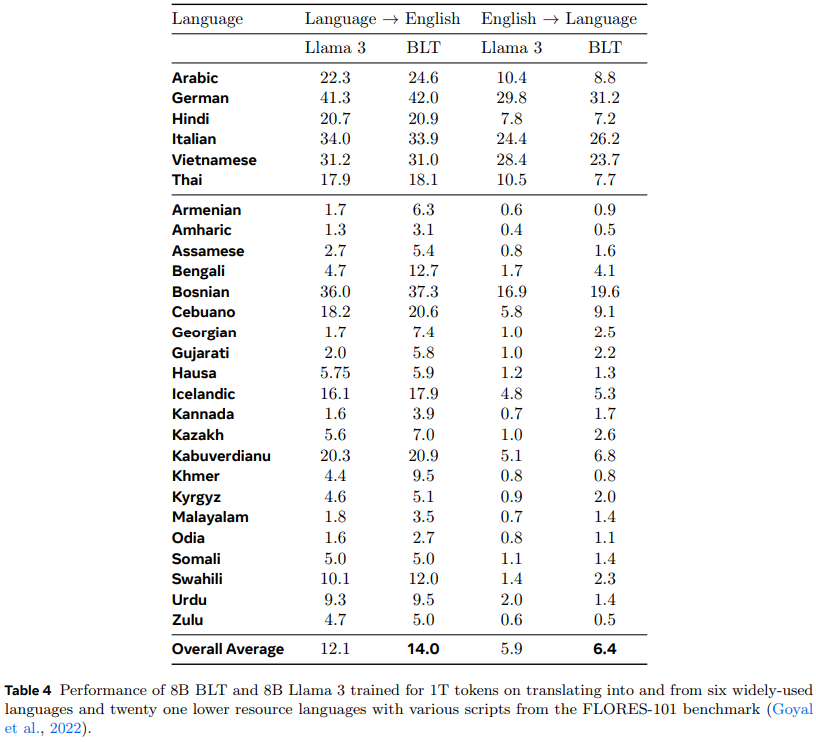
\includegraphics[height=0.9\textheight,width=1.05\textwidth,keepaspectratio]{images/recent-advance/blt-performance.png}
    \end{figure}
\framebreak
    \begin{figure}
        \centering
        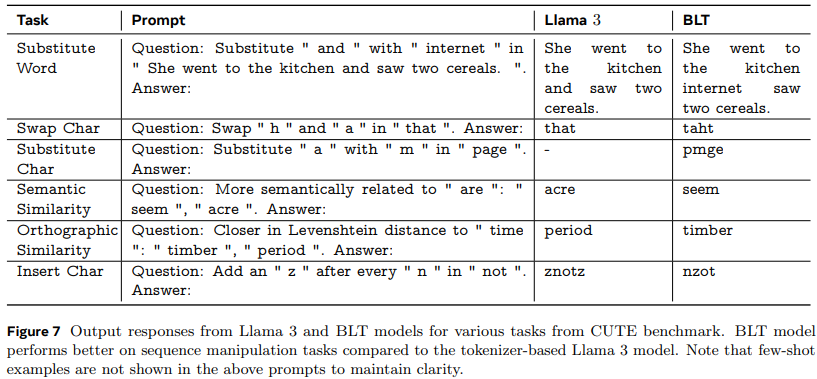
\includegraphics[height=0.9\textheight,width=1.05\textwidth,keepaspectratio]{images/recent-advance/blt-llama-3.png}
    \end{figure}
\end{frame}